\documentclass{beamer}
\mode <presentation>
{
    \usetheme{boxes}
    \usecolortheme{crane}
    \setbeamercovered{transparent}
}
\definecolor{craneorange}{RGB}{220,197, 90}

\usepackage{pgf,pgfarrows,pgfnodes}
\usepackage[english]{babel}
\usepackage{times}
\usepackage{amsmath}
% math extension - one probably wants to use symbols like '[' (written as '$[$')
\usepackage{ucs}
%\usepackage[utf8]{inputenc}
\usefonttheme{structuresmallcapsserif}

% utf8x does not work with xetex
\usepackage{ifxetex}
\ifxetex
\else
        \usepackage[utf8x]{inputenc}
\fi

\usepackage[normalem]{ulem}

%\setbeamercolor{background canvas}{bg=
\includegraphics[width=\textwidth]{./pics/wolf.png}}

\title{IT asset management with GLPI}
\author{\href{http://www.FusionInventory.org}{FusionInventory.org}}
\subject{IT asset management with FusionInventory and GLPI}
\keywords{IT asset management, Inventory, FusionInventory, GLPI}

\date{LinuxTag 2011}
\titlegraphic{GLPI and FusionInventory}
%subtitle{
\includegraphics[width=1.2cm]{./pics/fusioninventory-logo.png}}
\institute{
\includegraphics[height=3.2cm]{./pics/logos/Logo_LinuxTag.pdf}}
\author{ Gonéri Le Bouder and Walid Nouh }
\logo{
\includegraphics[height=0.7cm]{./pics/logos/glpi+fusinv_small.jpg}}

\AtBeginSection[] % Do nothing for \section*
{
    \begin{frame}<beamer>
        \frametitle{Outline}
    \tableofcontents[currentsection]
        \end{frame}
}


%%%%%%%%%%%%%%%%%%%%%%%%%%%%%%%%%%%%%%%%%%%%%%%
%%%%%%%%%%%%%%%%%%%%%%%%%%%%%%%%%%%%%%%%%%%%%%%
\begin{document}

\frame[plain]{\titlepage}

\begin{frame}
    \frametitle{About us: Walid Nouh}

    \begin{block}{IT management consultant}
        \begin{itemize}
        \item GLPI core developer
        \item FusionInventory project co-leader
        \item Rollerskate fanatic
        \item Work at TECLIB', Brussels, Belgium
        \end{itemize}
    \end{block}

\end{frame}



\begin{frame}
    \frametitle{About us: Gonéri Le Bouder}


    \begin{block}{Free software enthusiast}
        \begin{itemize}
        \item Debian Developer
        \item Perl Monger
        \item Former OCS Inventory developer
        \item FusionInventory project co-leader
        \item Work at TECLIB', Paris, France
        \item {\tiny and an awful french accent}
        \end{itemize}
    \end{block}

\end{frame}


\section{What is GLPI for?}


\begin{frame}
    \frametitle{What is GLPI for?}

 \begin{columns}
 \begin{column}{0.35\textwidth}
         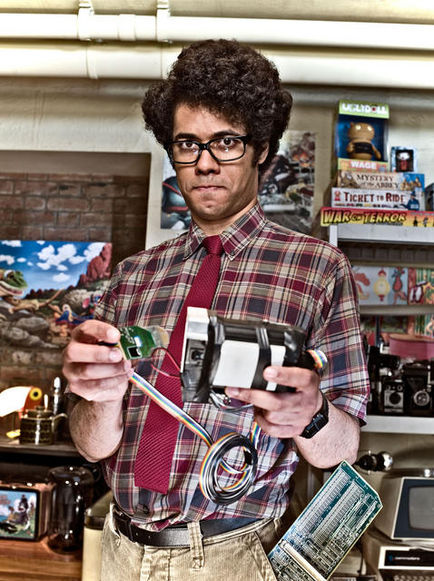
\includegraphics[height=7.5cm]{./pics/itcrowd.jpg}
 \end{column}
 \begin{column}{0.65\textwidth}
    \begin{block}{The IT crowd}
        \begin{itemize}
            \item How many server still run with 2GB of memory?
            \item Do we still have those old Toshiba laptops?
            \item Do our servers have the lastest security fixes?
        \end{itemize}
    \end{block}
 \end{column}
\end{columns}

 \end{frame}

\begin{frame}
    \frametitle{What is GLPI for?}

 \begin{columns}
 \begin{column}{0.1\textwidth}
         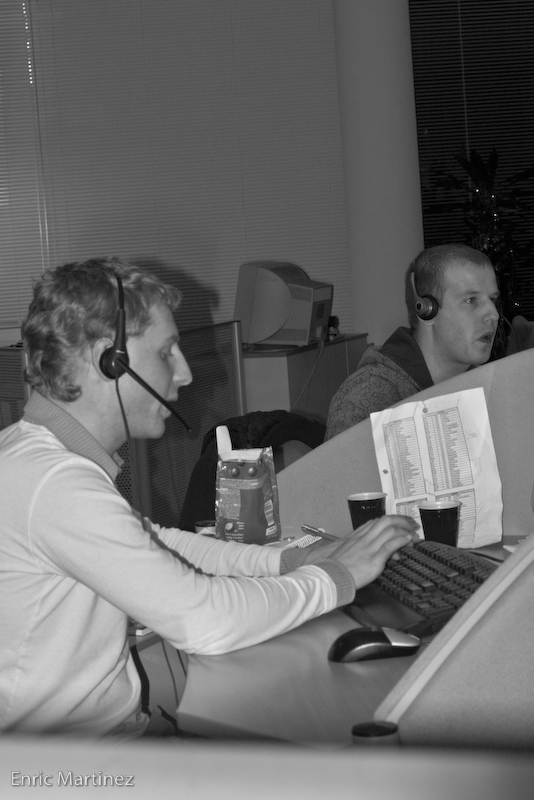
\includegraphics[height=7.5cm]{./pics/helpdesk.jpg}
 \end{column}
 \begin{column}{1\textwidth}

    \begin{block}{The Service Desk team}
        \begin{itemize}
            \item Is Mr Smith computer's harddrive full?
            \item What is my intervention planning?
            \item The printer ink cartridge is running \\
                low on the second floor!
        \end{itemize}
    \end{block}
 \end{column}
\end{columns}


\end{frame}

\begin{frame}
    \frametitle{What is GLPI for?}

 \begin{columns}
 \begin{column}{0.35\textwidth}
         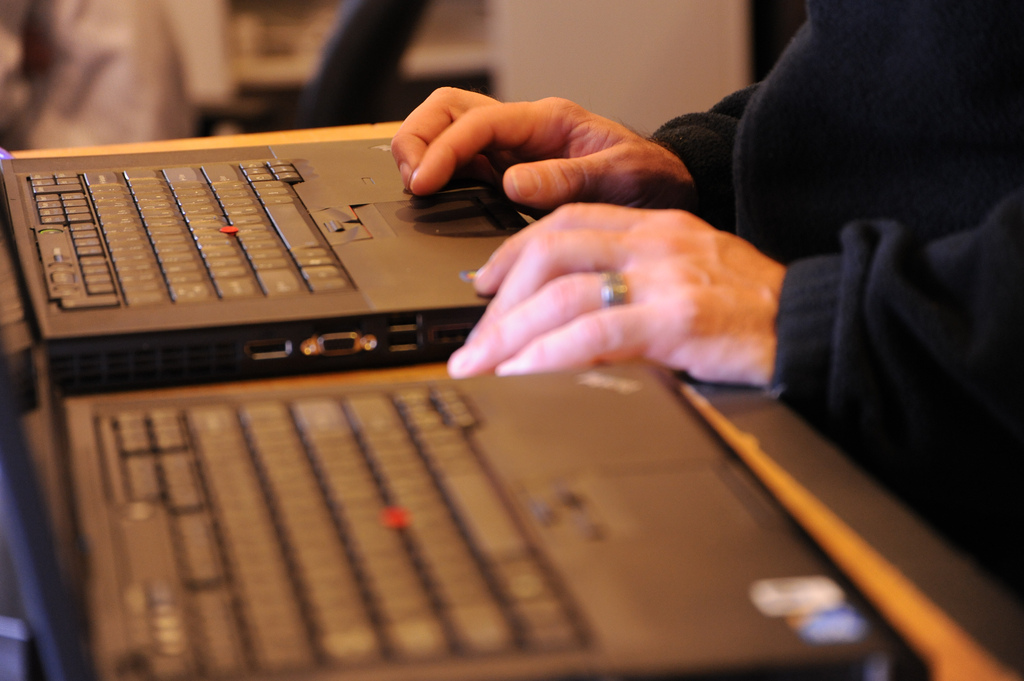
\includegraphics[height=7.5cm]{./pics/lenovo.jpg}
 \end{column}
 \begin{column}{0.65\textwidth}

    \begin{block}{The users}
        \begin{itemize}
            \item Why can't I print?
            \item Why can't I send email anymore?
            \item Are the IT guys really processing my request?
        \end{itemize}
    \end{block}
 \end{column}
\end{columns}

\end{frame}

\begin{frame}
    \frametitle{What is GLPI for?}

 \begin{columns}
 \begin{column}{0.15\textwidth}
         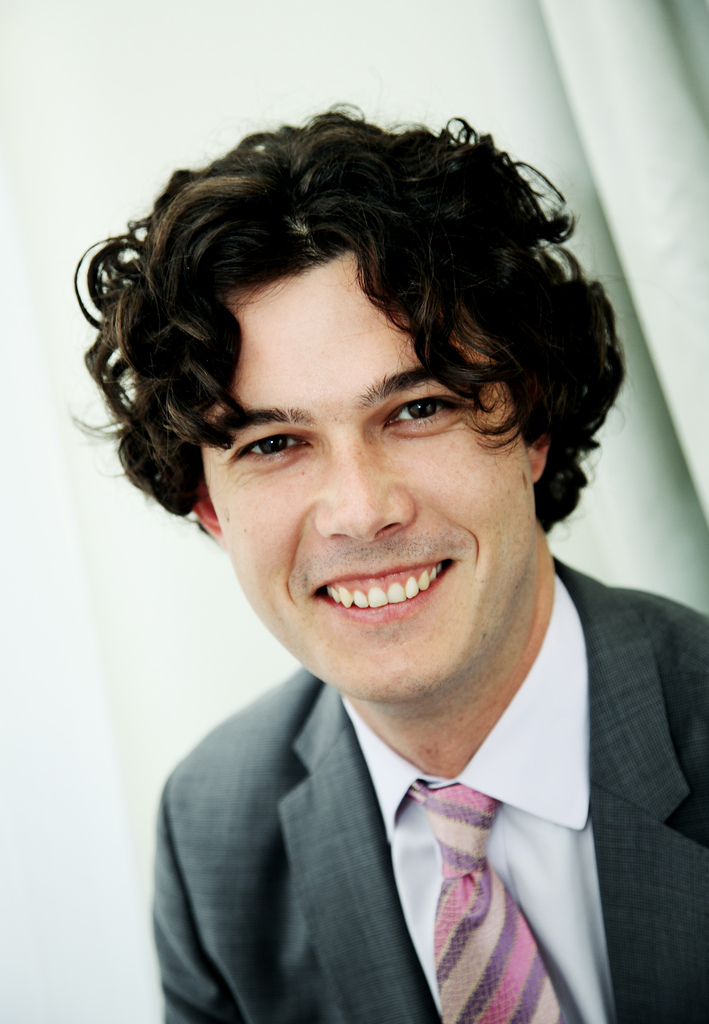
\includegraphics[height=8.5cm]{./pics/manager.jpg}
 \end{column}
 \begin{column}{1.25\textwidth}
    \begin{block}{The management}
        \begin{itemize}
            \item How many request per day processed by our support team?
            \item What is our users satisfaction's level?
            \item I need more dashboards!
        \end{itemize}
    \end{block}
 \end{column}
\end{columns}


\end{frame}


\begin{frame}
    \frametitle{What is GLPI for?}

 \begin{columns}
 \begin{column}{0.35\textwidth}
         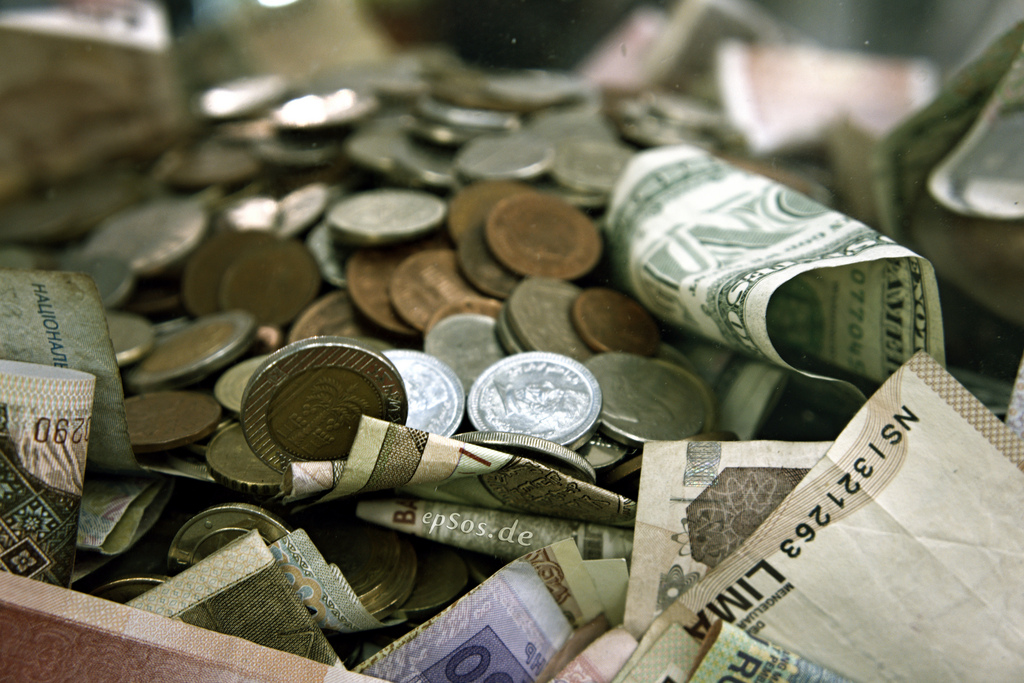
\includegraphics[height=7.5cm]{./pics/purchasing.jpg}
 \end{column}
 \begin{column}{0.65\textwidth}
    \begin{block}{The purchasing department}
        \begin{itemize}
            \item How much did we spend last year with IBM?
            \item Is the paternship with Oracle still running?
            \item How many and where are the assets bought with last year budget?
        \end{itemize}
    \end{block}
 \end{column}
\end{columns}
\end{frame}


\section{Installation / Architecture?}


\begin{frame}
    \frametitle{Installation}

         \pgfputat{\pgfxy(-1,-3)}{\pgfbox[left,top]{
\includegraphics[height=2.5cm]{./pics/php-mysql.jpg}}}
    \begin{block}{Easy step}
        \begin{itemize}
            \item Common web application
            \item Very few OS dependencies
        \end{itemize}
    \end{block}

    Extract, run the wizard, your done!

\end{frame}

\begin{frame}
    \frametitle{Architecture}

 \begin{columns}
 \begin{column}{0.34\textwidth}
 \end{column}
 \begin{column}{0.90\textwidth}
    
\includegraphics[height=6.5cm]{pics/scale.pdf}
 \end{column}
\end{columns}

\end{frame}

\begin{frame}
    \frametitle{Architecture}

 \begin{columns}
 \begin{column}{0.34\textwidth}
    \begin{block}{Really?}
        \begin{itemize}
            \item Existing large installation of GLPI \\
            {\small up to 130K computers inventoried}
            \item 1 million computers referenced so far and still growing
        \end{itemize}
    \end{block}

 \end{column}
 \begin{column}{0.90\textwidth}
    
\includegraphics[height=6.5cm]{pics/scale.pdf}

 \end{column}
\end{columns}

\end{frame}


\section{Collect your informations}

\begin{frame}
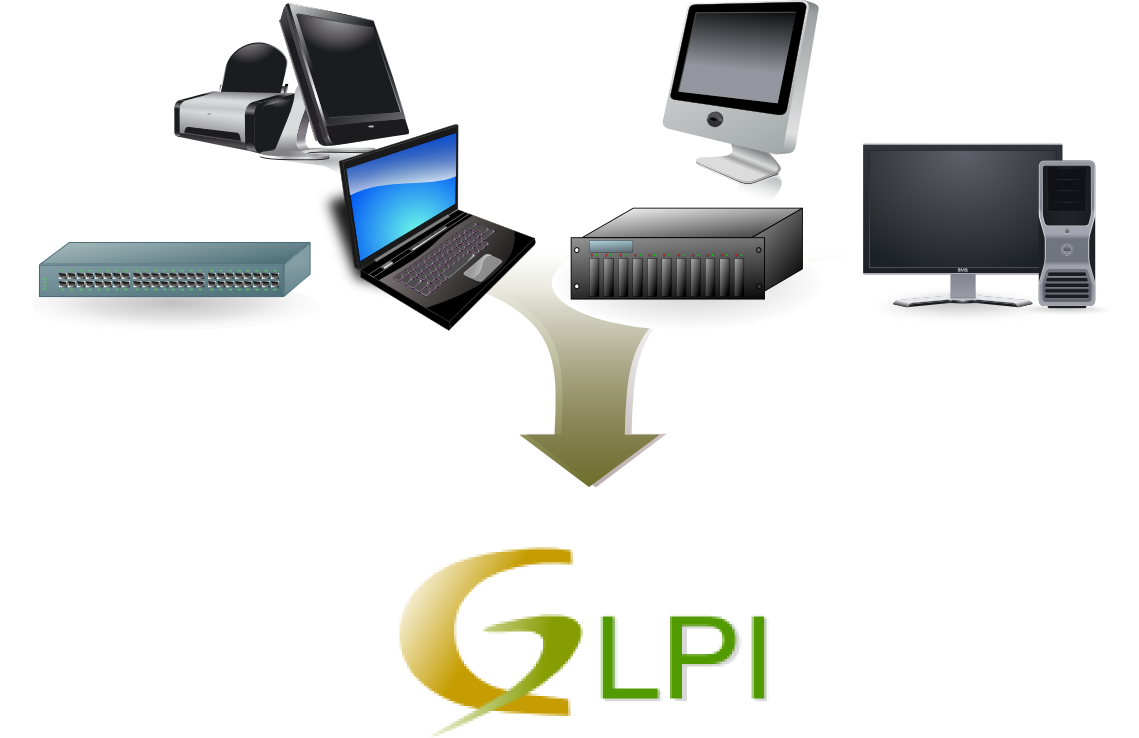
\includegraphics[height=6.5cm]{pics/bigpicture.png}
\end{frame}


\begin{frame}

    \frametitle{Collect your information}

 \begin{columns}
 \begin{column}{0.34\textwidth}
    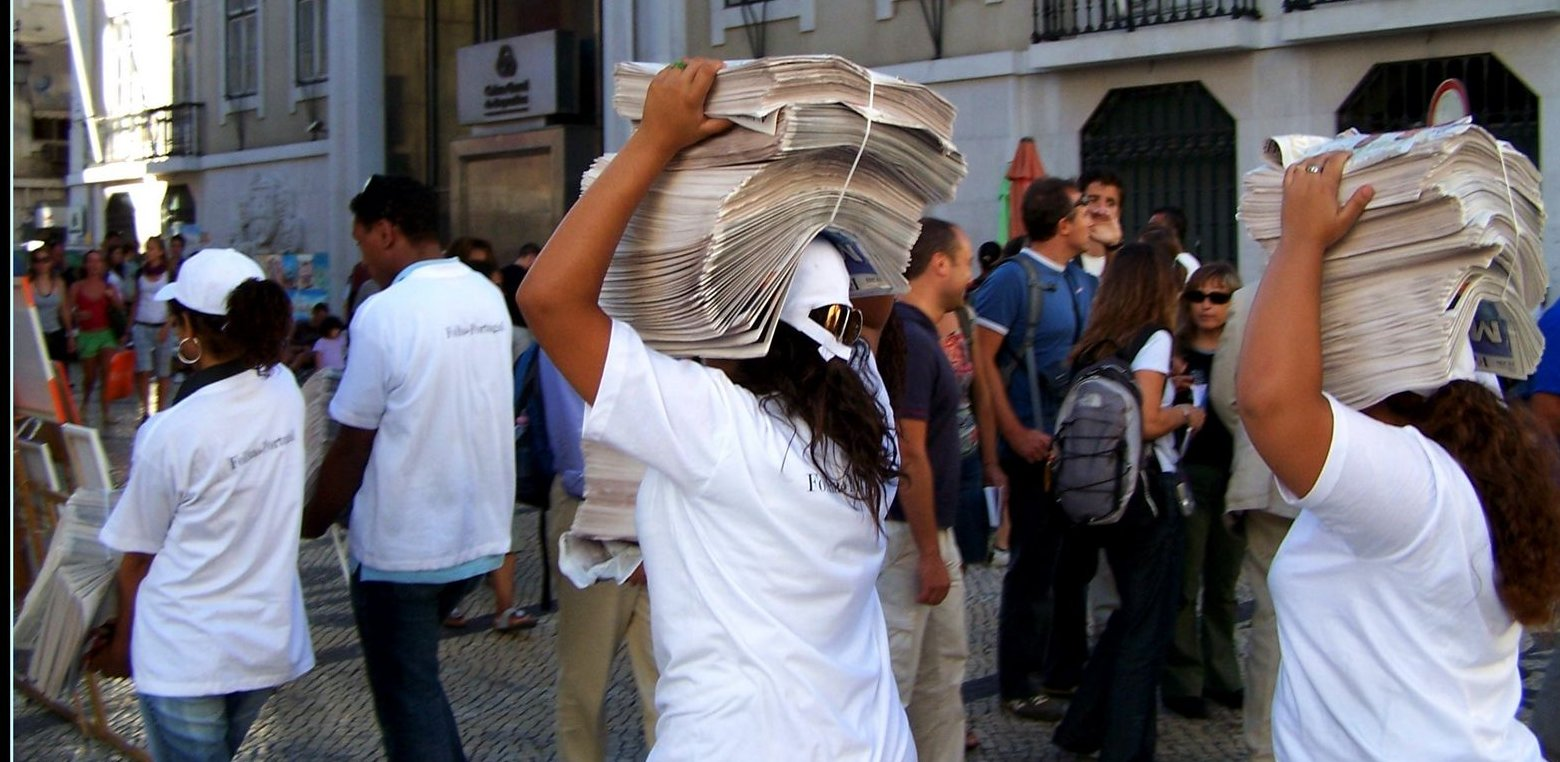
\includegraphics[height=6.5cm]{pics/information.jpg}
 \end{column}
 \begin{column}{0.90\textwidth}
 \end{column}
\end{columns}


\end{frame}



\begin{frame}

    \frametitle{Collect your information}

 \begin{columns}
 \begin{column}{0.34\textwidth}
    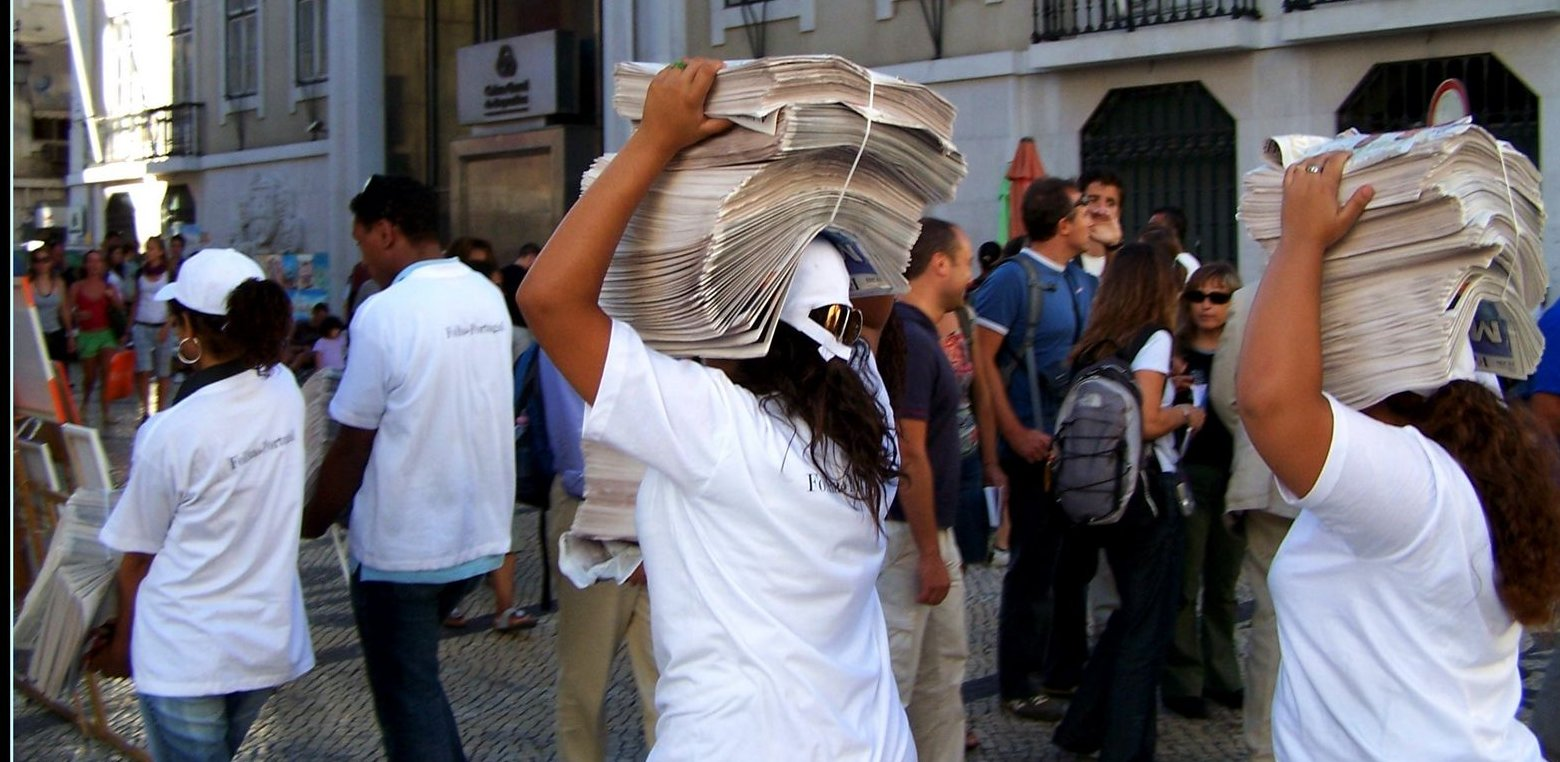
\includegraphics[height=6.5cm]{pics/information.jpg}
 \end{column}
 \begin{column}{0.90\textwidth}
    \begin{block}{Inputs}
        \begin{itemize}
            \item Desktop computers and server
            \item Network devices
            \item Data coming from legacy systems
            \item Financial informations
            \item ...
        \end{itemize}
    \end{block}

 \end{column}
\end{columns}


\end{frame}

\begin{frame}

    \frametitle{Computer}
 \begin{columns}
 \begin{column}{0.15\textwidth}
         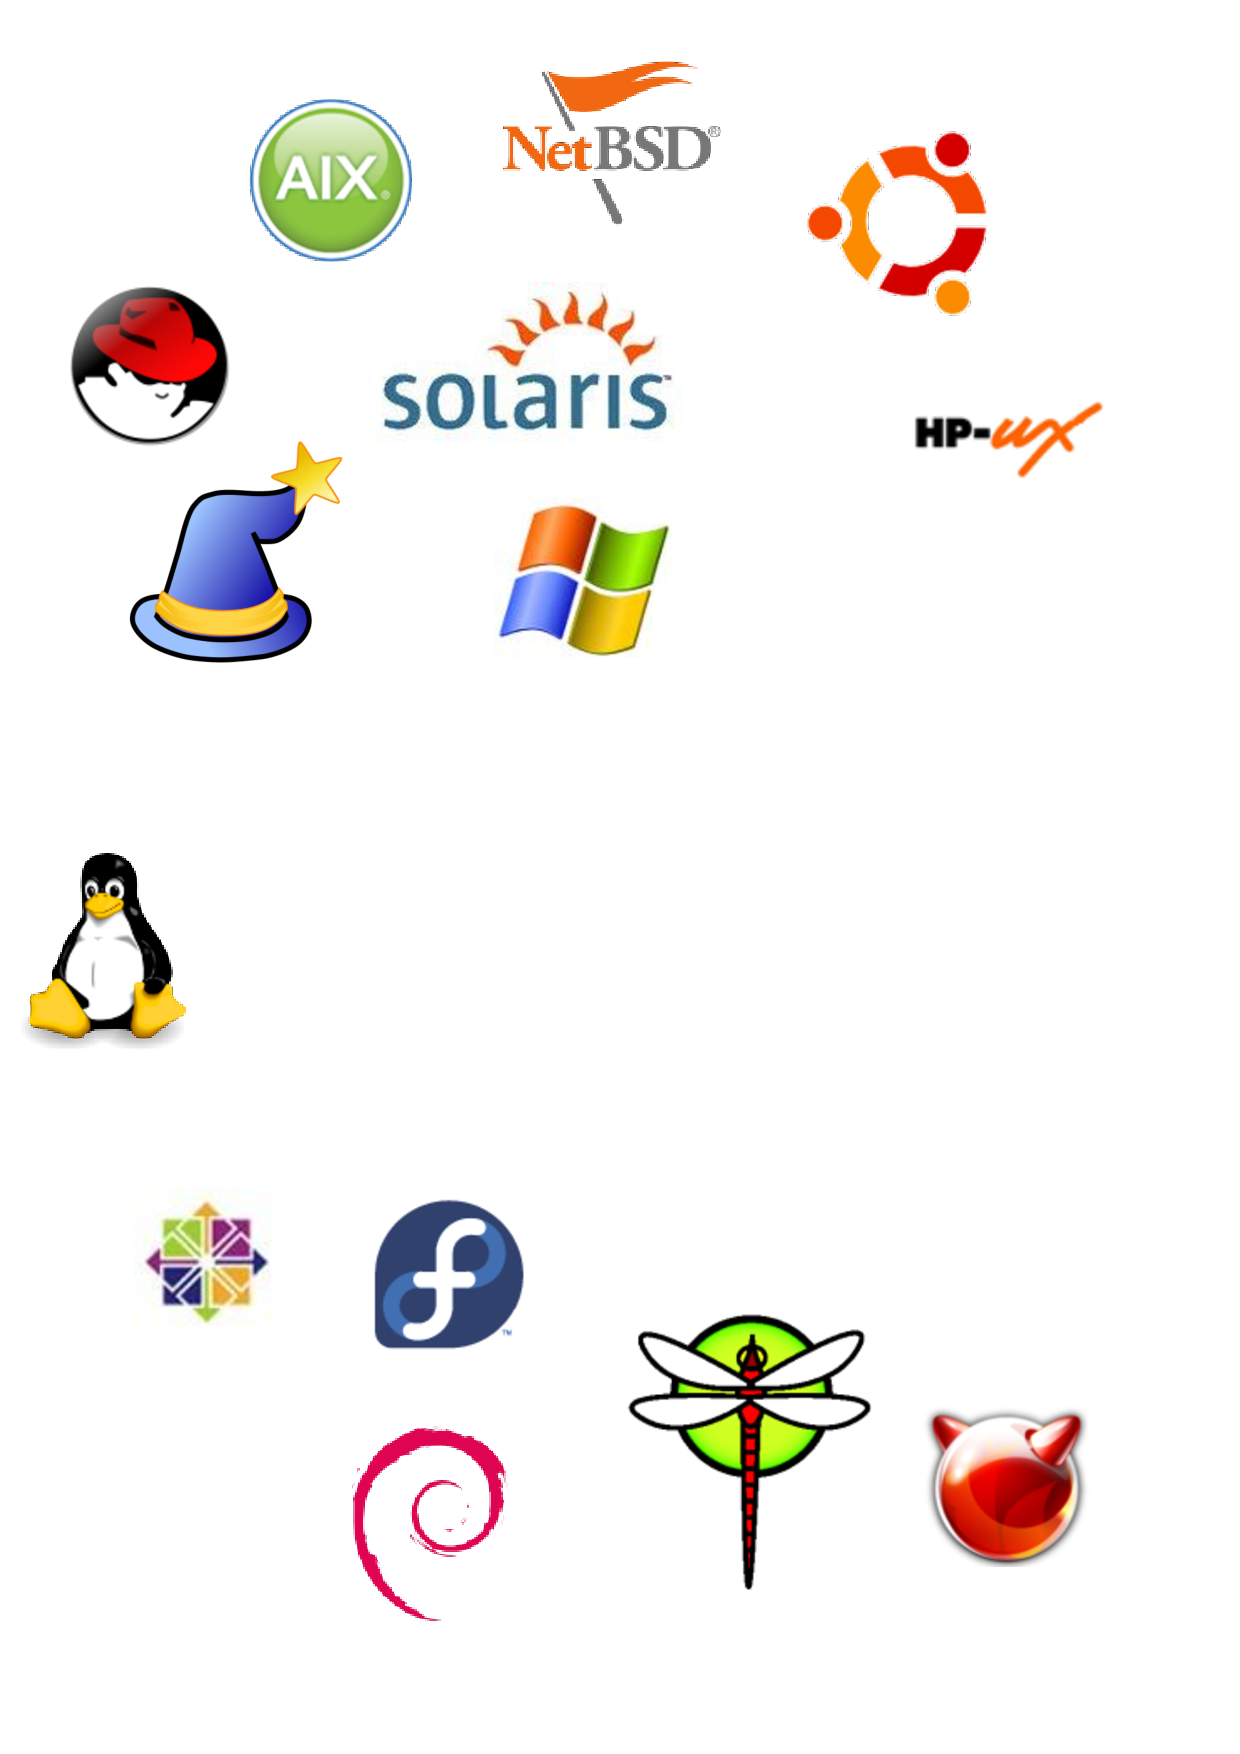
\includegraphics[height=8.5cm]{./pics/os.pdf}
 \end{column}
 \begin{column}{1.25\textwidth}
    \begin{block}{Easy step}
        \begin{itemize}
            \item Agent packaged for most of the OSes
            \item Ready to use, no build, no dependency!
        \end{itemize}
    \end{block}


 \end{column}
\end{columns}




\end{frame}

\begin{frame}

    \frametitle{Network devices}


 \begin{columns}
 \begin{column}{0.15\textwidth}
         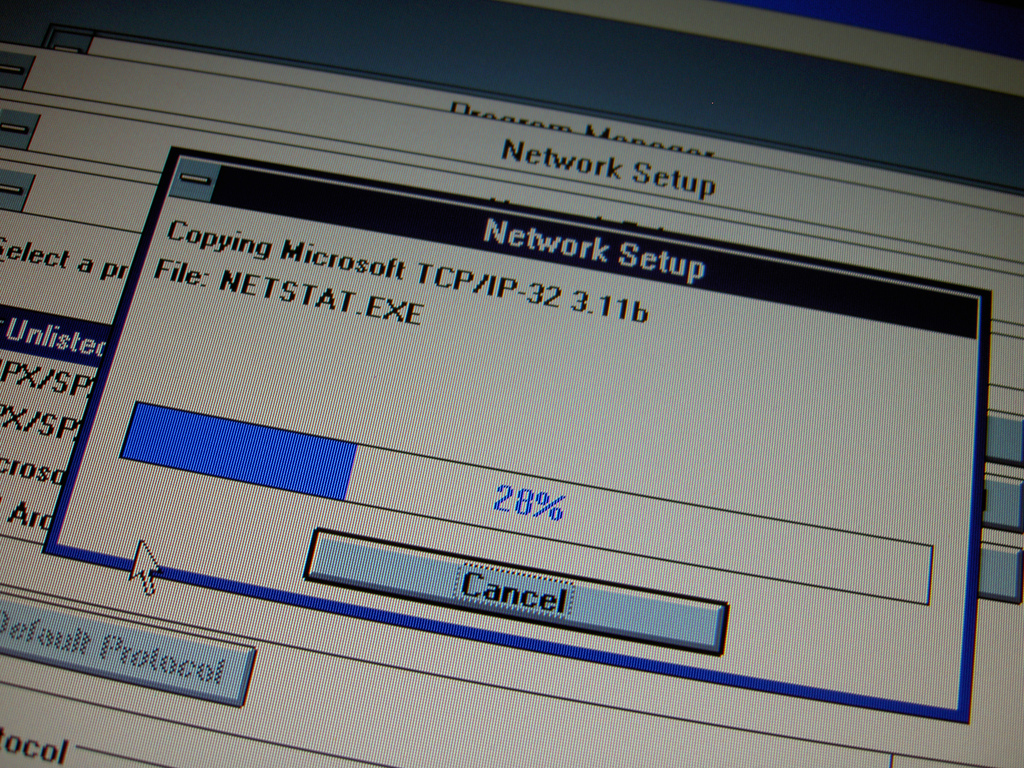
\includegraphics[height=8.5cm]{./pics/networking.jpg}
 \end{column}
 \begin{column}{1.25\textwidth}
    

    \begin{block}{Routers, switchs, printers... \\
    FusionInventory do it remotely for you}
        \begin{itemize}
            \item Nothing to install
            \item Network scan to identify asset
            \item Use SNMP to collect information
        \end{itemize}
    \end{block}

 \end{column}
\end{columns}
\end{frame}


\begin{frame}

    \frametitle{Network devices}


 \begin{columns}
 \begin{column}{0.15\textwidth}
         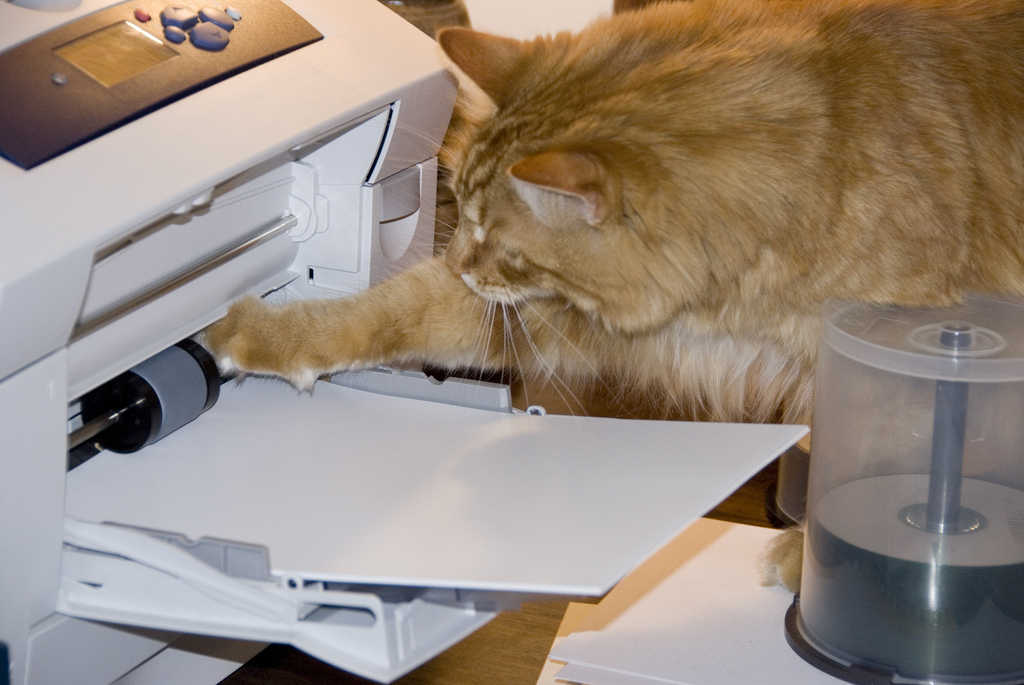
\includegraphics[height=8.5cm]{./pics/printer.jpg}
 \end{column}
 \begin{column}{1.25\textwidth}
    

    \begin{block}{printers}
        \begin{itemize}
            \item Cartridge ink levels
            \item Counters and statistics
        \end{itemize}
    \end{block}

 \end{column}
\end{columns}
\end{frame}



\section{Integration}

\begin{frame}

    \frametitle{Existing systems}

 
    \begin{block}{What about my current system?}
        \begin{itemize}
            \item Financial informations
            \item Licenses
            \item Helpdesk
        \end{itemize}
    \end{block}
   

\end{frame}

\begin{frame}

    \frametitle{Application integration}
 \begin{columns}
 \begin{column}{0.45\textwidth}
         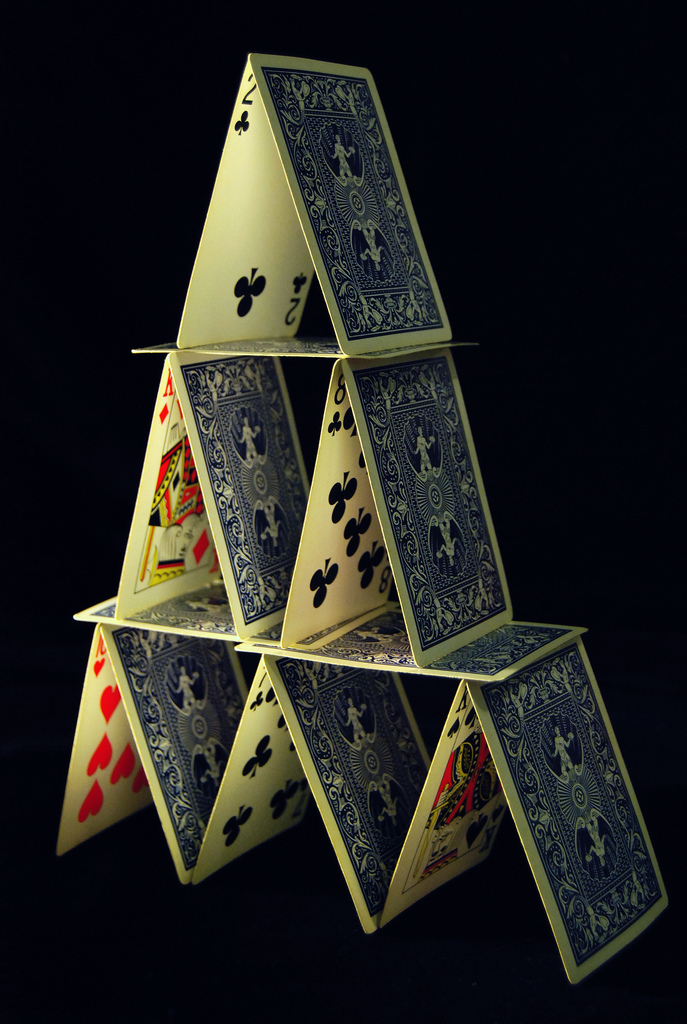
\includegraphics[height=7.5cm]{./pics/house_of_cards.jpg}
 \end{column}
 \begin{column}{0.45\textwidth}
     \begin{block}{Wait, some tools are already running here! \\
     How to interacte with them?}
        \begin{itemize}
            \item Webservice interface
            \item API for updates
            \item CSV import/export
        \end{itemize}
    \end{block}
   
 \end{column}
\end{columns}
\end{frame}


\begin{frame}

    \frametitle{Application integration: plugins}

 \begin{columns}
 \begin{column}{0.45\textwidth}
         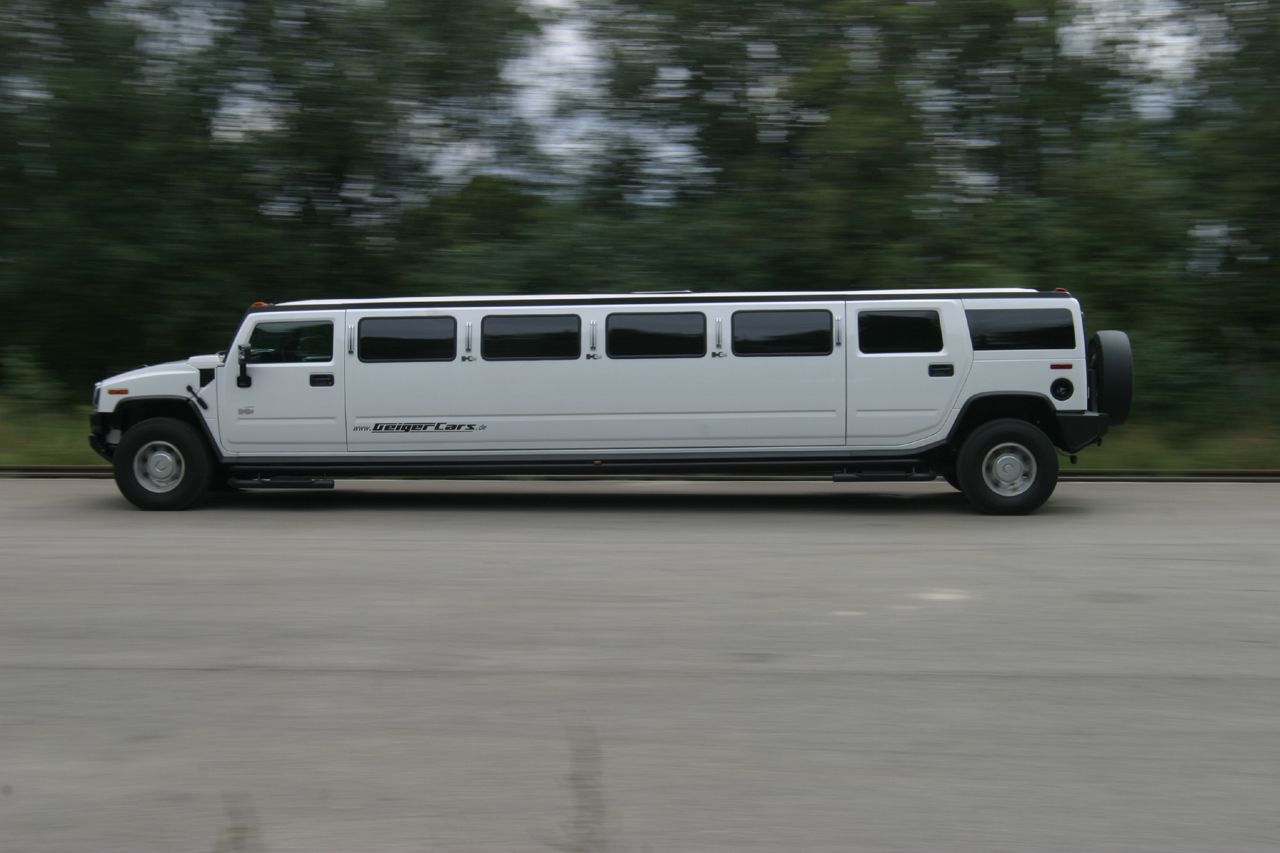
\includegraphics[height=7.5cm]{./pics/plugin.jpg}
 \end{column}
 \begin{column}{0.65\textwidth}
    \begin{block}{A large collection of \\
    extensions}
        \begin{itemize}
            \item Add load of new features
            \item Tight integration in GLPI
            \item Powerfull API
        \end{itemize}
    \end{block}

 \end{column}
\end{columns}





\end{frame}


\begin{frame}


    \frametitle{GLPI, all in one}
 \begin{columns}
 \begin{column}{0.45\textwidth}
         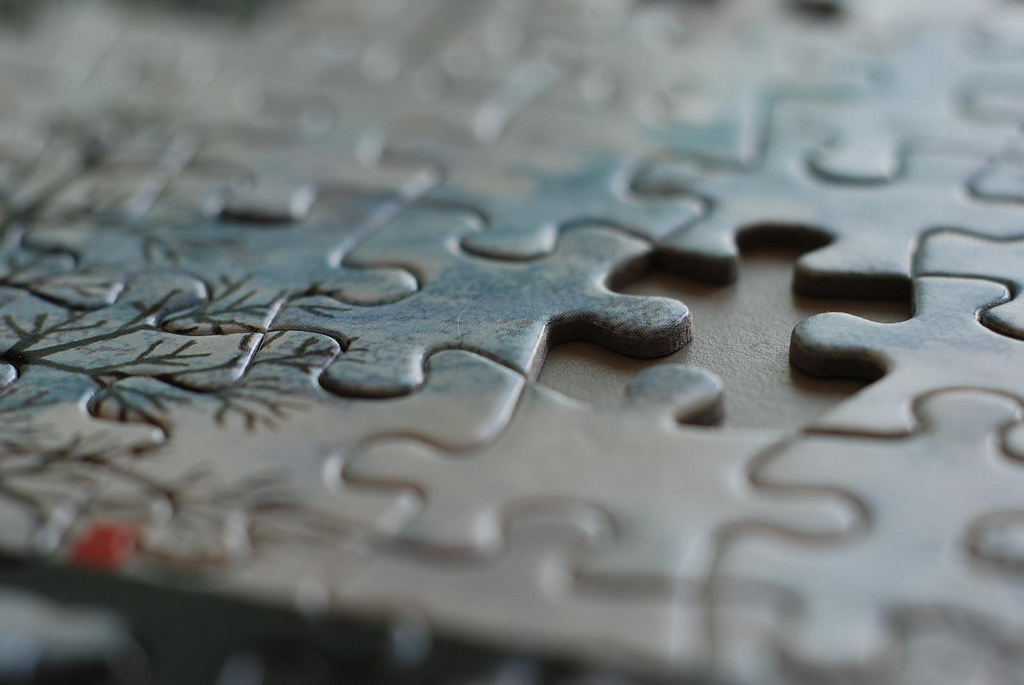
\includegraphics[height=7.5cm]{./pics/glpithelink.jpg}
 \end{column}
 \begin{column}{0.65\textwidth}
    \begin{block}{The asset timeline}
        \begin{itemize}
            \item Past : history
            \item Current : inventory
            \item Future : warranty, contracts
        \end{itemize}

    \end{block}

 \end{column}
\end{columns}
\end{frame}


\begin{frame}


    \frametitle{GLPI, all in one}
 \begin{columns}
 \begin{column}{0.45\textwidth}
         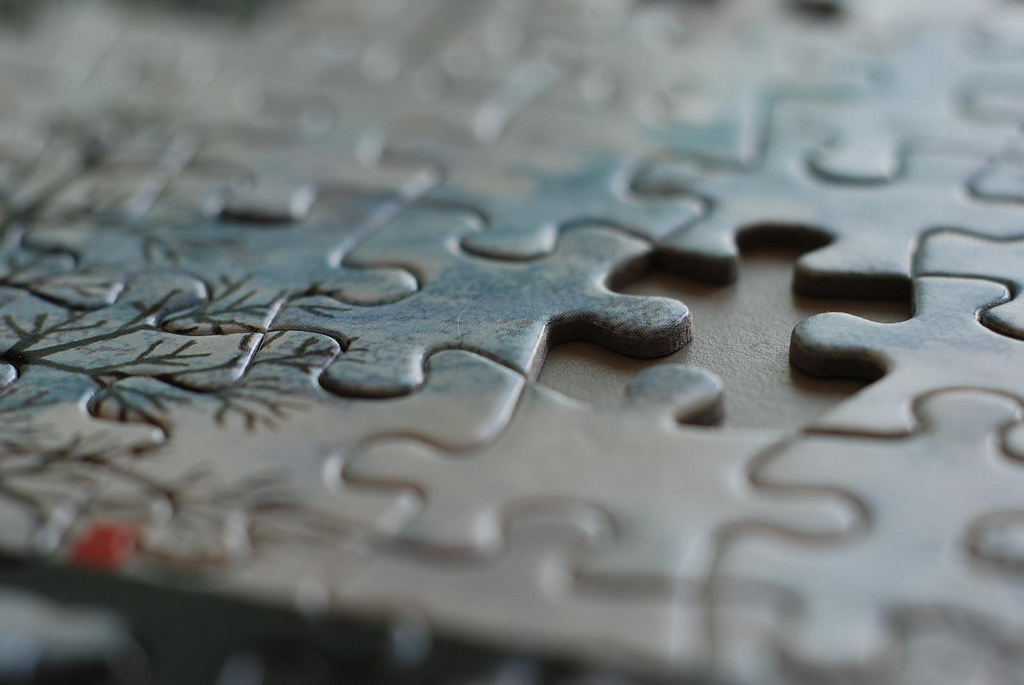
\includegraphics[height=7.5cm]{./pics/glpithelink.jpg}
 \end{column}
 \begin{column}{0.65\textwidth}
    \begin{block}{Helpdesk for everyone}
        \begin{itemize}
            \item Tickets on assets
        \end{itemize}

    \end{block}

 \end{column}
\end{columns}
\end{frame}

\begin{frame}


    \frametitle{GLPI, all in one}
 \begin{columns}
 \begin{column}{0.45\textwidth}
         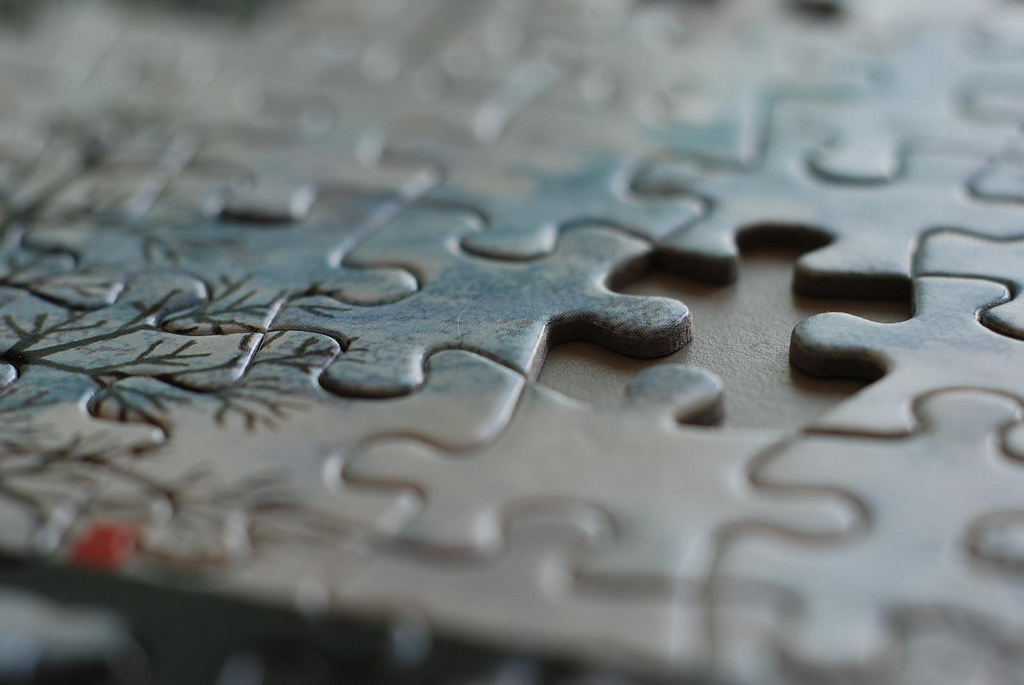
\includegraphics[height=7.5cm]{./pics/glpithelink.jpg}
 \end{column}
 \begin{column}{0.65\textwidth}
    \begin{block}{Accurate statistics}
        \begin{itemize}
            \item 25\% of last year laptops have harddrive failure !
            \item How many incidents are resolved by using VNC  ? 
        \end{itemize}

    \end{block}

 \end{column}
\end{columns}
\end{frame}

\section{Authorisation}

\begin{frame}
    \frametitle{Authorisation}


 \begin{columns}
 \begin{column}{0.34\textwidth}
    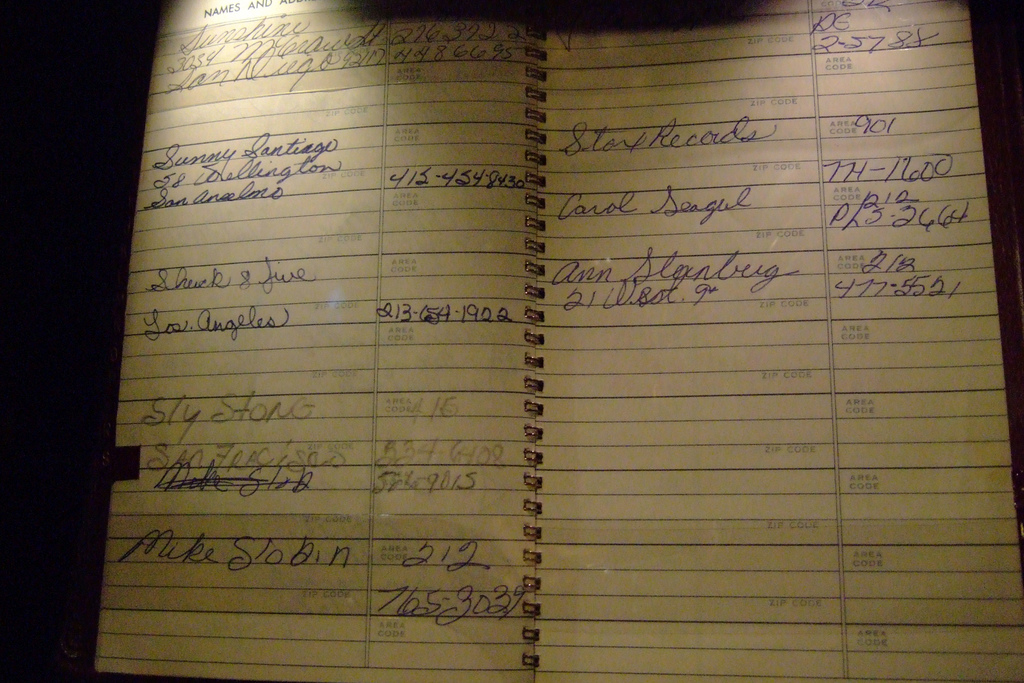
\includegraphics[height=6.5cm]{pics/addressbook.jpg}
 \end{column}
 \begin{column}{0.90\textwidth}
    \begin{block}{Native LDAP support}
        \begin{itemize}
            \item Strong LDAP integration
            \item LDAP v3 compatible \\
            {\small ActiveDirectory, OpenLDAP, ...}
        \end{itemize}
    \end{block}

    \begin{block}{Other authentication methods}
        \begin{itemize}
            \item POP3
            \item IMAP
        \end{itemize}
    \end{block}
 \end{column}
\end{columns}
\end{frame}

\begin{frame}
    \frametitle{Authorisation}


 \begin{columns}
 \begin{column}{0.34\textwidth}
    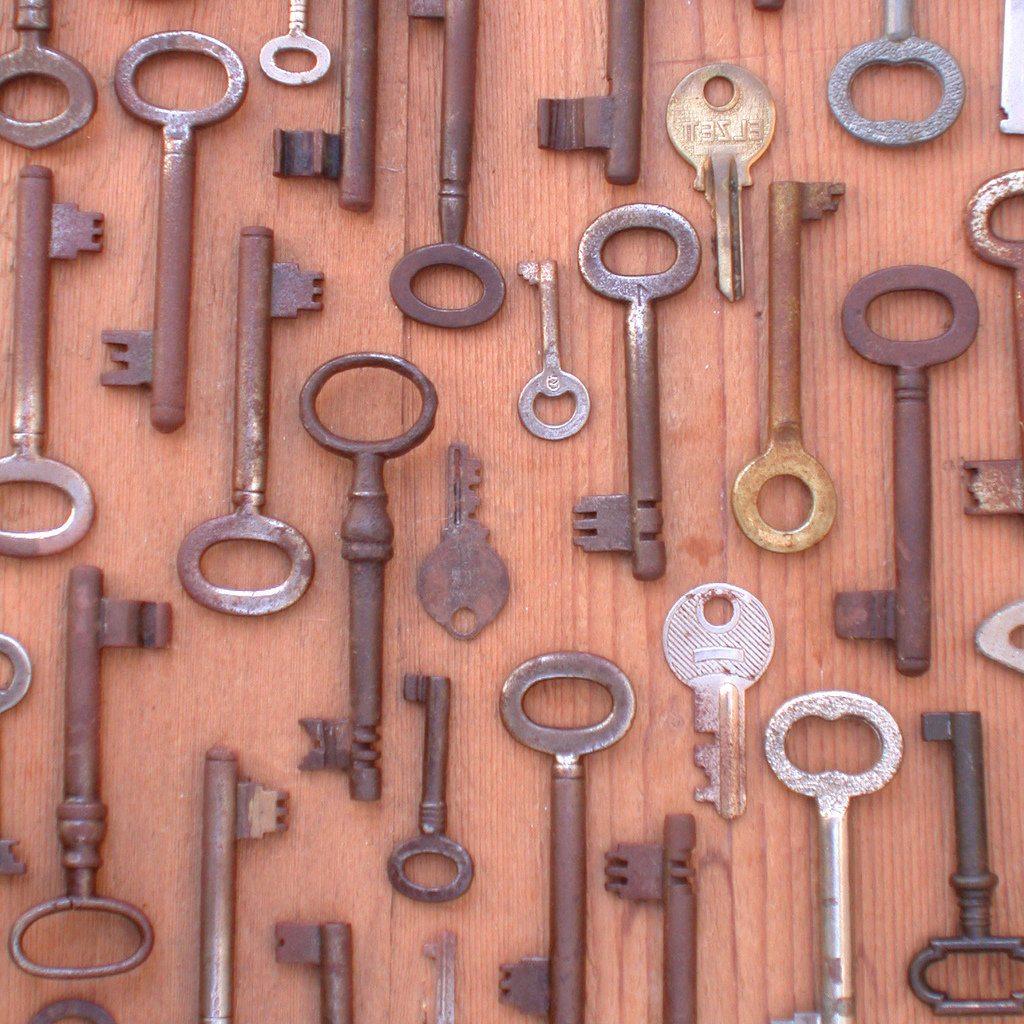
\includegraphics[height=10.5cm]{pics/sso.jpg}
 \end{column}
 \begin{column}{0.90\textwidth}
    \begin{block}{Single Sign On too!}
        \begin{itemize}
            \item WebSSO
            \item CAS
        \end{itemize}
    \end{block}
 \end{column}
\end{columns}

\end{frame}




\begin{frame}
\frametitle{Authorisation}
    \begin{block}{Entities}
        \begin{itemize}
            \item Independent administrative entity
            \item Can be mapped on your LDAP organisation
            \item Contain assets and tickets
        \end{itemize}

    \end{block}
\end{frame}

\begin{frame}
\frametitle{Habilitations: organizational chart}
\begin{columns}
 \begin{column}{0.45\textwidth}
         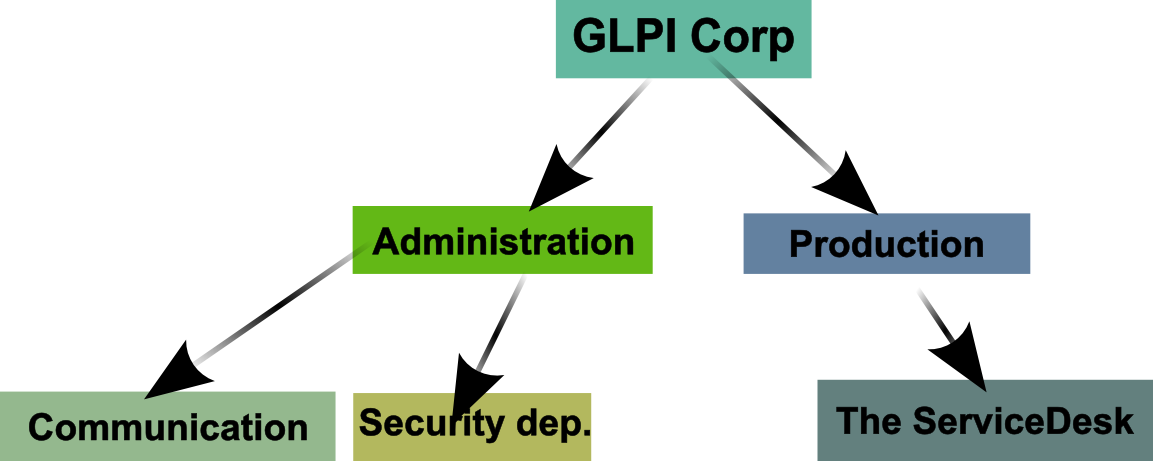
\includegraphics[height=4.5cm]{./pics/entites.png}
 \end{column}
 \begin{column}{0.45\textwidth}
 \end{column}
\end{columns}
\end{frame}





\begin{frame}
\frametitle{Authorisation}
    \begin{block}{Profile}
        \begin{itemize}
            \item More than 100 rights
            \item Habilitation : a profile on an entity 
        \end{itemize}
    \end{block}
\end{frame}


\begin{frame}
\frametitle{Authorisation: Example}
Let's take an example.
\end{frame}

\begin{frame}
\frametitle{Entities: Example}
\begin{columns}
 \begin{column}{0.45\textwidth}
         
\includegraphics[height=7.5cm]{./pics/simpsons/mayor_Joe-Quimby.png}
 \end{column}
 \begin{column}{0.45\textwidth}
    \begin{block}{The CEO}
        \begin{itemize}
            \item Manage the company 
        \end{itemize}

    \end{block}

 \end{column}
\end{columns}
\end{frame}

\begin{frame}
\frametitle{Authorisation: Example}
\begin{columns}
 \begin{column}{0.45\textwidth}
         
\includegraphics[height=7.5cm]{./pics/simpsons/Montgomery_Burns.png}
 \end{column}
 \begin{column}{0.45\textwidth}
    \begin{block}{The CTO}
        \begin{itemize}
            \item Can do whatever he wants in the IT department
        \end{itemize}
    \end{block}
 \end{column}
\end{columns}
\end{frame}

\begin{frame}
\frametitle{Authorisation: Example}
\begin{columns}
 \begin{column}{0.45\textwidth}
         
\includegraphics[height=7.5cm]{./pics/simpsons/comm_kent_brockman.png}
 \end{column}
 \begin{column}{0.45\textwidth}
    \begin{block}{Press officer}
        \begin{itemize}
            \item Watches everything
            \item Generates charts and dashboards
        \end{itemize}
    \end{block}
 \end{column}
\end{columns}
\end{frame}

\begin{frame}
\frametitle{Authorisation: Example}
\begin{columns}
 \begin{column}{0.45\textwidth}
         
\includegraphics[height=7.5cm]{./pics/simpsons/police_Wiggum_Clancy.png}
 \end{column}
 \begin{column}{0.45\textwidth}
    \begin{block}{Security officer}
        \begin{itemize}
            \item Regulates the processes
            \item Can have a look on everything 
        \end{itemize}
    \end{block}
 \end{column}
\end{columns}
\end{frame}


\begin{frame}
\frametitle{Authorisation: Example}
\begin{columns}
 \begin{column}{0.45\textwidth}
         
\includegraphics[height=7.5cm]{./pics/simpsons/homer.png}
 \end{column}
 \begin{column}{0.45\textwidth}
    \begin{block}{The support engineer}
        \begin{itemize}
            \item Can only sees and answers users requests
        \end{itemize}
    \end{block}
 \end{column}
\end{columns}
\end{frame}



\begin{frame}
\frametitle{Authorisation: Profile}
\begin{columns}
 \begin{column}{0.45\textwidth}
         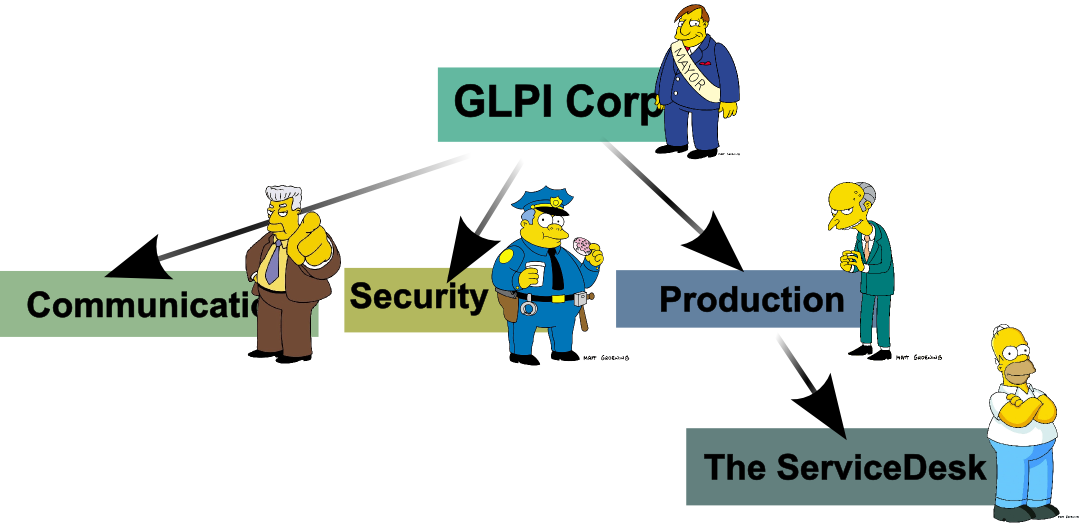
\includegraphics[height=4.5cm]{./pics/entites-ppl.png}
 \end{column}
 \begin{column}{0.45\textwidth}
 \end{column}
\end{columns}
\end{frame}

\section{Service Desk}

\begin{frame}
\frametitle{Service Desk: the big picture}
\begin{columns}
\begin{column}{0.45\textwidth}
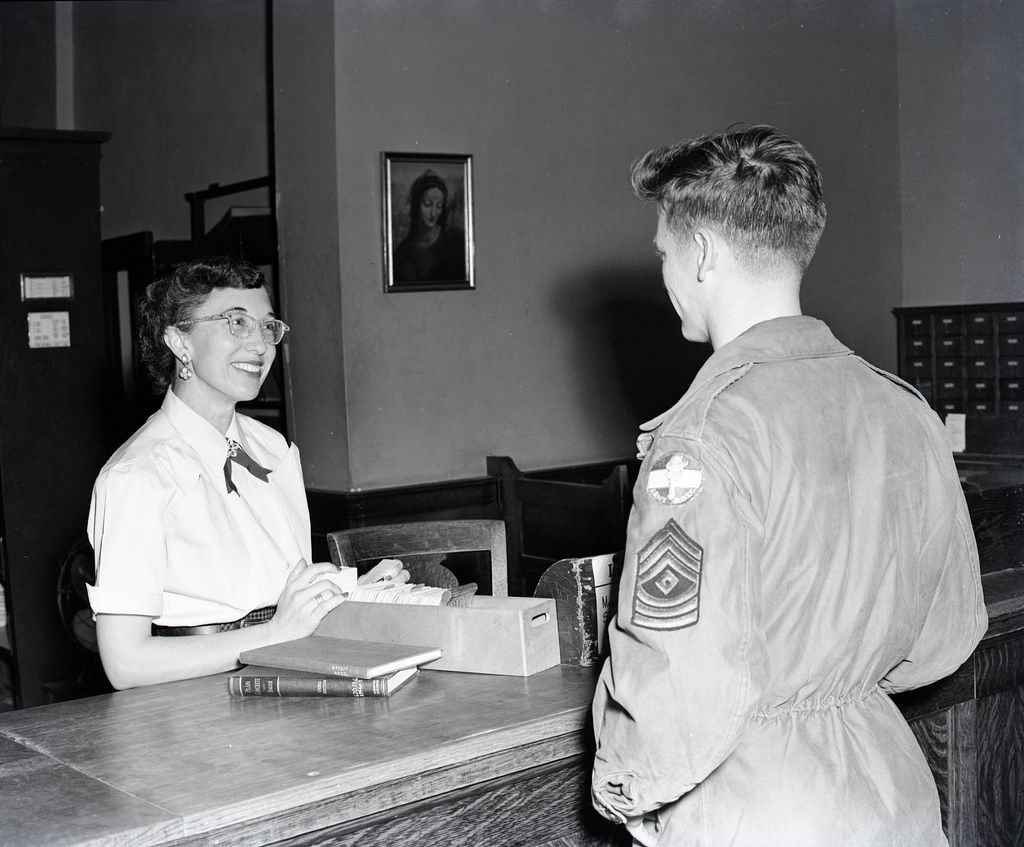
\includegraphics[height=7.5cm]{./pics/servicedesk.jpg}
\end{column}
\begin{column}{0.45\textwidth}
\end{column}
\end{columns}
\end{frame}



\begin{frame}


    \frametitle{Service Desk: the big picture}
 \begin{columns}
 \begin{column}{0.45\textwidth}
         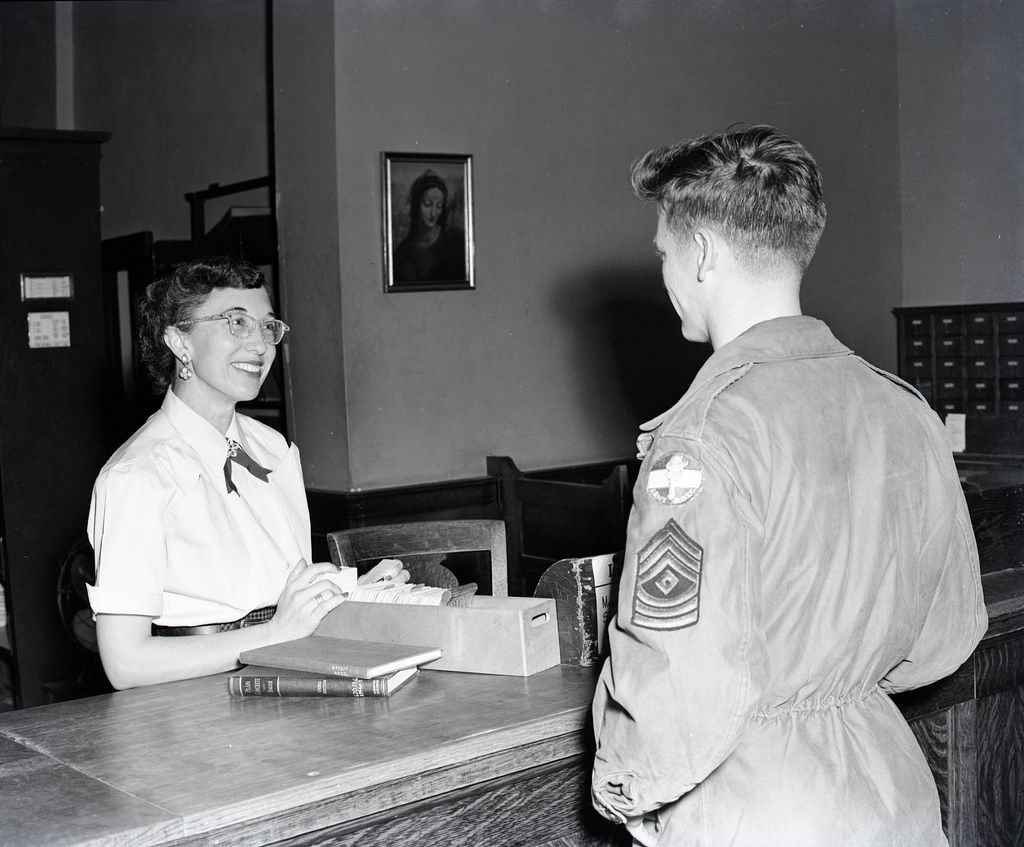
\includegraphics[height=7.5cm]{./pics/servicedesk.jpg}
 \end{column}
 \begin{column}{0.45\textwidth}
    \begin{block}{ITIL v1 compliant}
        \begin{itemize}
            \item SLA
            \item user satisfaction
            \item Incident management
            \item Business rules
            \item Notifications, multilingual support
        \end{itemize}

    \end{block}
   
 \end{column}
\end{columns}
\end{frame}

\begin{frame}

    \frametitle{Service Desk: the interfaces 1/2}

 \begin{columns}
 \begin{column}{0.45\textwidth}
         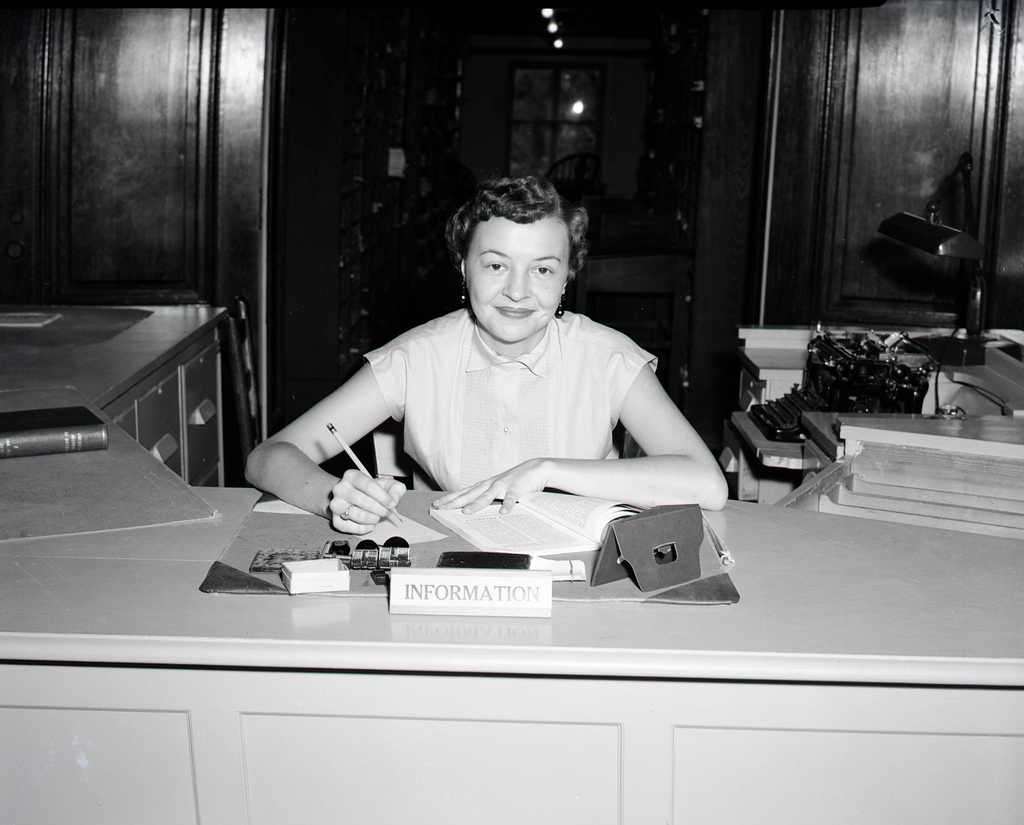
\includegraphics[height=7.5cm]{./pics/servicedesk2.jpg}
 \end{column}
 \begin{column}{0.45\textwidth}
     \begin{block}{Web interfaces}
        \begin{itemize}
            \item End user simplified interface
            \item Standard interface
            \item Smartphones interface
        \end{itemize}
    \end{block}
  
 \end{column}
\end{columns}






\end{frame}
\begin{frame}

    \frametitle{Service Desk: the interfaces 2/2}


 \begin{columns}
 \begin{column}{0.45\textwidth}
         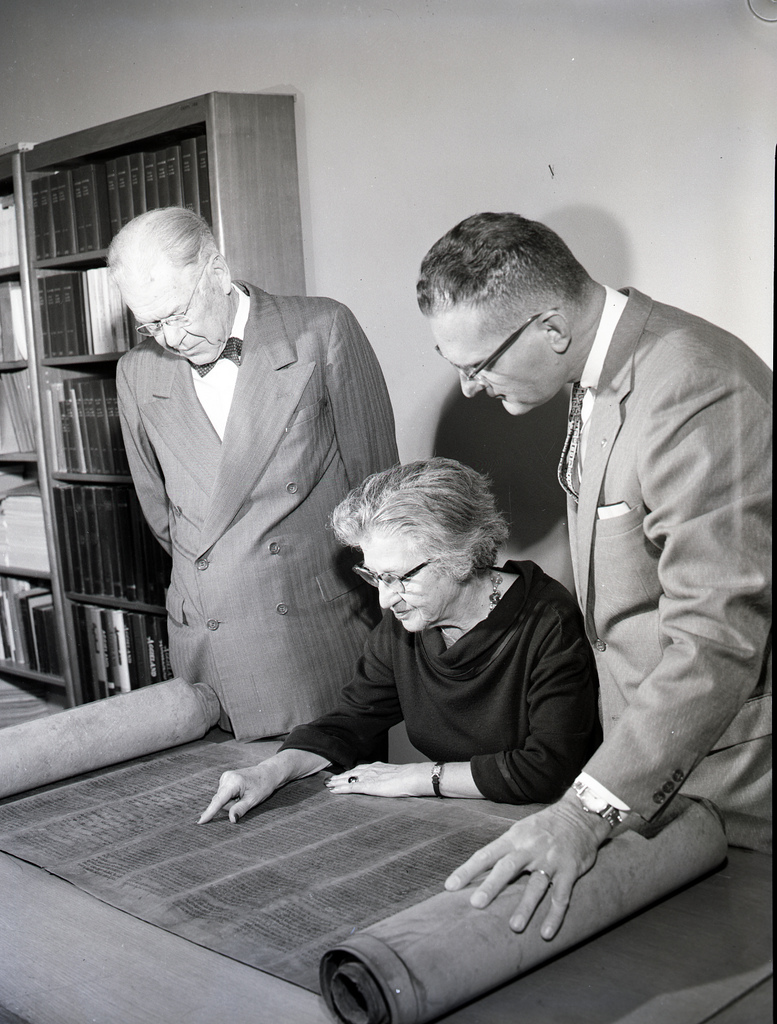
\includegraphics[height=7.5cm]{./pics/servicedesk3.jpg}
 \end{column}
 \begin{column}{0.45\textwidth}
     \begin{block}{Webservices}
        \begin{itemize}
            \item To integrate GLPI in another system
            \item To push tickets into another helpdesk software
            \item Or the opposite
        \end{itemize}
    \end{block}
\pause
    \begin{block}{Mail}
       \begin{itemize}
            \item Send notifications
            \item Add and update tickets
       \end{itemize}
    \end{block}

 
 \end{column}
\end{columns}

\end{frame}

\begin{frame}

\frametitle{Service Desk: reporting}
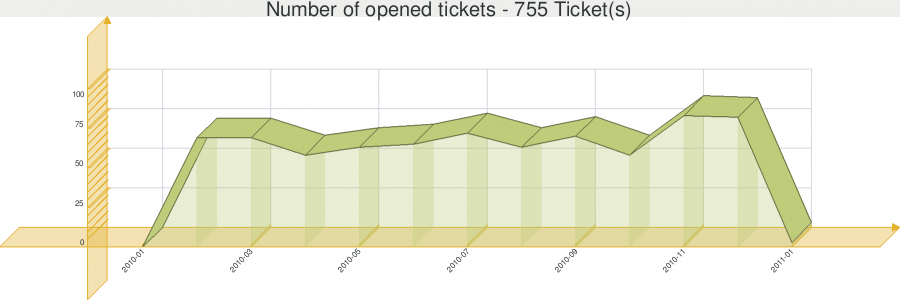
\includegraphics[height=3.5cm]{./pics/report1.png}
\end{frame}

\section{What else}

\begin{frame}

    \frametitle{What Else?}


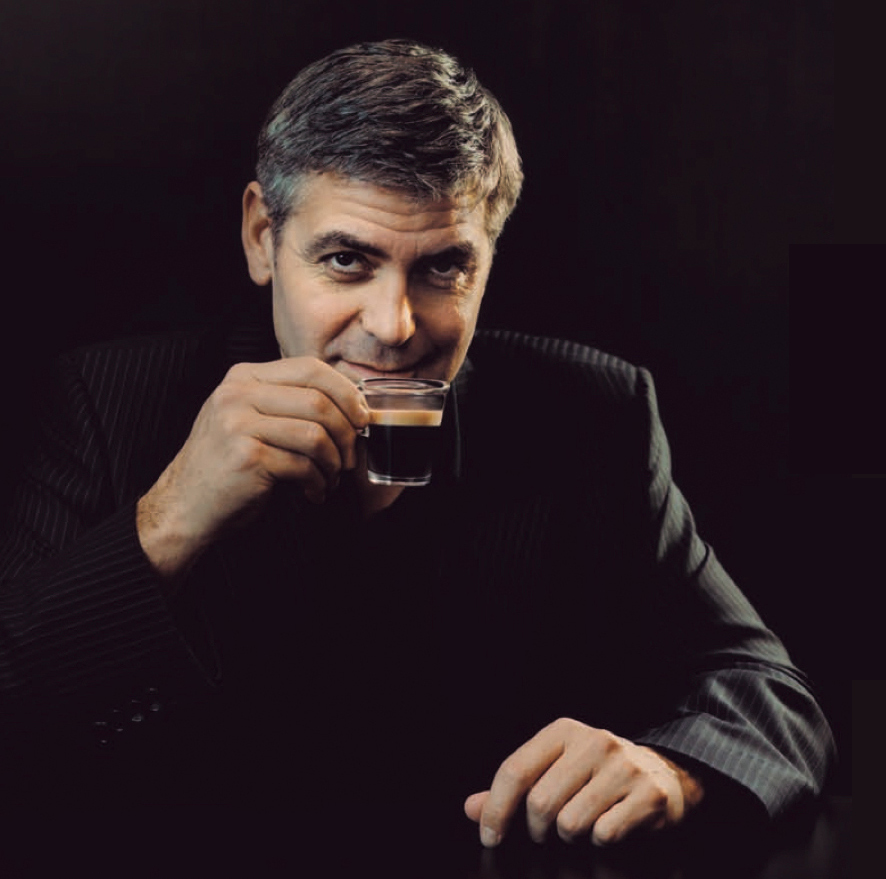
\includegraphics[height=7.5cm]{./pics/whatelse.jpg}

\end{frame}

\begin{frame}

    \frametitle{GLPI}

    \begin{block}{A nonprofit organisation}
        \begin{itemize}
            \item Indepnet, a french nonprofit association
            \item Since 2002
        \end{itemize}
    \end{block}

\end{frame}

\begin{frame}

    \frametitle{GLPI}

    \begin{block}{Two independant projects leaders}
        \begin{itemize}
            \item Jean-Mathieu Doléans
            \item Julien Dombre
        \end{itemize}
    \end{block}
\pause
    \begin{block}{Contributors and developers}
        \begin{itemize}
            \item Developers and contributors
            \item Plugins developers
            \item Translators
        \end{itemize}
    \end{block}

\end{frame}

\begin{frame}

    \frametitle{GLPI}

 \begin{columns}
 \begin{column}{0.35\textwidth}
         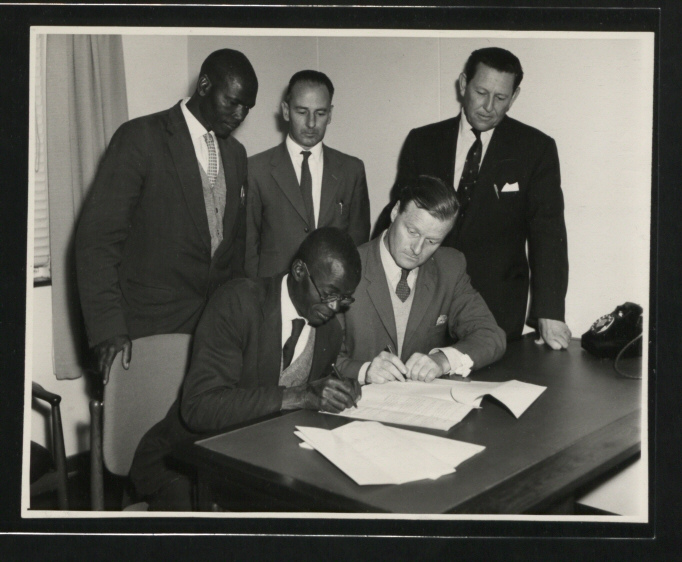
\includegraphics[height=7.5cm]{./pics/agreement.jpg}
 \end{column}
 \begin{column}{0.65\textwidth}

    \begin{block}{GLPI Business partners}
        \begin{itemize}
            \item Agreement between the association and IT partners
            \item Partners bring money, support and code
        \end{itemize}
    \end{block}


 \end{column}
\end{columns}

\end{frame}

\begin{frame}

    \frametitle{FusionInventory}

    \begin{block}{A sister project}
        \begin{itemize}
            \item Created by some people of the GLPI community
            \item Strong relationship with GLPI
        \end{itemize}
    \end{block}
\pause
    \begin{block}{A community}
        \begin{itemize}
            \item More than 10 people involved
            \item Supported by 2 companies
        \end{itemize}
    \end{block}
\pause
    \begin{block}{But also}
        \begin{itemize}
            \item Open minded : other projects are welcomed!
            \item Agent already used by third party projects
        \end{itemize}
    \end{block}

\end{frame}

\section{Questions}

\begin{frame}
    \frametitle{Thanks}

        \begin{itemize}
                \item Purchasing: \url{http://www.flickr.com/photos/epsos/5394616925/}
                \item LDAP: \url{http://www.flickr.com/photos/heyrocker/2954514315/}
                \item SSO: \url{http://www.flickr.com/photos/13519089@N03/1380483002/}
                \item User picture: \url{http://www.flickr.com/photos/wonderlane/5043174502/}
                \item Manager: \url{http://www.flickr.com/photos/eastcapital/5228405457/}
                \item Server: \url{http://www.flickr.com/photos/sylvar/31436963/}
                \item Helpdesk: \url{http://www.flickr.com/photos/runlevel0/2196587153/}
                \item Database: \url{http://www.flickr.com/photos/garryknight/5476230085/}
                \item Information: \url{http://www.flickr.com/photos/garryknight/5476230085/}
                \item Networking: \url{http://www.flickr.com/photos/dbreg2007/4376127852/}
                \item Printer: \url{http://www.flickr.com/photos/photofarmer/467241015/}
                \item House of cards: \url{http://www.flickr.com/photos/gibbons/2294375187/in/photostream/}
                \item Sercice desk: \url{http://www.flickr.com/photos/cushinglibrary/4770917261/}
        \end{itemize}

\end{frame}



\end{document}
